% ============================================================
%  CUGA FLO: Towards Agentic Business Process Management via
%  the Task–Decision–Flow Model
% ============================================================
\documentclass[11pt,a4paper]{article}

% ── Packages ─────────────────────────────────────────────────────────────────
\usepackage[margin=1in]{geometry}
\usepackage[T1]{fontenc}
\usepackage[utf8]{inputenc}
\usepackage{lmodern}
\usepackage{microtype}
\usepackage{amsmath,amssymb,amsthm}
\usepackage{booktabs}
\usepackage{graphicx}
\usepackage{xcolor}
\usepackage{listings}
\usepackage{hyperref}
\usepackage{enumitem}
\usepackage{parskip}
\usepackage{caption}
\usepackage{subcaption}
\usepackage{tikz}
\usetikzlibrary{shapes.geometric,arrows.meta,positioning,fit,backgrounds,calc,patterns}
\usepackage{float}
\usepackage{algorithm}
\usepackage{algpseudocode}
\usepackage{mdframed}
\usepackage{authblk}
\usepackage{multirow}
\usepackage{array}
\usepackage{tabularx}
\usepackage{setspace}
\usepackage{footmisc}

% ── Theorem environments ──────────────────────────────────────────────────────
\newtheorem{definition}{Definition}
\newtheorem{theorem}{Theorem}
\newtheorem{proposition}{Proposition}
\newtheorem{remark}{Remark}

% ── Hyperref ─────────────────────────────────────────────────────────────────
\hypersetup{
  colorlinks=true,
  linkcolor=blue!55!black,
  citecolor=blue!55!black,
  urlcolor=blue!55!black,
}

% ── Code listings ─────────────────────────────────────────────────────────────
\definecolor{codebg}{rgb}{0.96,0.96,0.96}
\definecolor{codegreen}{rgb}{0.0,0.42,0.0}
\definecolor{codepurple}{rgb}{0.42,0.0,0.52}
\definecolor{codeorange}{rgb}{0.7,0.28,0.0}
\definecolor{codered}{rgb}{0.7,0.0,0.0}

\lstdefinestyle{python}{
  backgroundcolor=\color{codebg},
  commentstyle=\color{codegreen}\itshape,
  keywordstyle=\color{codepurple}\bfseries,
  stringstyle=\color{codeorange},
  basicstyle=\ttfamily\small,
  breaklines=true,
  keepspaces=true,
  language=Python,
  showstringspaces=false,
  tabsize=4,
  frame=single,
  rulecolor=\color{black!20},
  xleftmargin=6pt, xrightmargin=6pt,
}
\lstdefinestyle{json}{
  backgroundcolor=\color{codebg},
  basicstyle=\ttfamily\small,
  breaklines=true,
  frame=single,
  rulecolor=\color{black!20},
  xleftmargin=6pt, xrightmargin=6pt,
  morestring=[b]",
  stringstyle=\color{codeorange},
}

% ── TikZ node styles ──────────────────────────────────────────────────────────
\tikzset{
  task/.style={rectangle, rounded corners=4pt, draw=black!60,
               fill=blue!12, minimum width=2.5cm, minimum height=0.95cm,
               font=\small, text centered, text width=2.3cm},
  gateway/.style={diamond, draw=black!60, fill=orange!18, aspect=1.7,
                  minimum width=1.4cm, font=\scriptsize, text centered},
  hook/.style={rectangle, rounded corners=2pt, draw=red!65, fill=red!8,
               minimum width=2.2cm, minimum height=0.75cm,
               font=\scriptsize\itshape, text centered, text width=2.0cm,
               densely dashed, line width=0.8pt},
  event/.style={circle, draw=black!60, fill=white,
                minimum size=0.65cm, font=\scriptsize},
  flow/.style={-{Stealth[length=5.5pt]}, thick, black!65},
  hookflow/.style={-{Stealth[length=5.5pt]}, thick, red!60, densely dashed},
  policy/.style={rectangle, rounded corners=2pt, draw=green!50!black,
                 fill=green!6, minimum width=1.8cm, minimum height=0.6cm,
                 font=\scriptsize, text centered, text width=1.7cm},
  agent/.style={rectangle, rounded corners=4pt, draw=purple!55,
                fill=purple!8, minimum width=2.6cm, minimum height=1cm,
                font=\small, text centered, text width=2.4cm},
  frame/.style={rectangle, rounded corners=6pt, draw=teal!60,
                fill=teal!5, line width=1.2pt},
}

% ── Framed boxes ─────────────────────────────────────────────────────────────
\newmdenv[linewidth=1pt,linecolor=blue!40,backgroundcolor=blue!3,
          innerleftmargin=8pt,innerrightmargin=8pt,
          innertopmargin=6pt,innerbottommargin=6pt,
          skipabove=8pt,skipbelow=8pt]{policybox}

\newmdenv[linewidth=1.2pt,linecolor=teal!55,backgroundcolor=teal!3,
          innerleftmargin=10pt,innerrightmargin=10pt,
          innertopmargin=8pt,innerbottommargin=8pt,
          skipabove=8pt,skipbelow=8pt]{tealframe}

% ── Title ─────────────────────────────────────────────────────────────────────
\title{%
  \textbf{Towards Agentic Business Process Management:}\\[6pt]
  \large CUGA FLO and the Task--Decision--Flow Model\\[4pt]
  \normalsize \textit{Process-Aware, Policy-Aware Agents with Runtime Flow Adaptation}
}
\author[1]{Lior Limonad}
\affil[1]{CUGA Research}
\date{May 2026}

% =============================================================================
\begin{document}
\maketitle
\thispagestyle{plain}

% ── Abstract ──────────────────────────────────────────────────────────────────
\begin{abstract}
We introduce \textbf{CUGA FLO}, the first realization of an \emph{Agentic Business
Process Management} (Agentic BPM) system, and the \textbf{Task--Decision--Flow
(TDF)} model that underpins it. Unlike conventional BPM systems, in which all
exception paths must be foreseen and encoded at design time, and unlike
LLM-as-planner approaches, in which an agent interprets a process description and
constructs an ad hoc execution plan without structural guarantees, CUGA FLO
introduces a third paradigm: a \emph{process-aware, policy-aware} \texttt{FlowAgent}
that governs the execution of a BPMN~2.0 process and adapts it at runtime through a
principled hook mechanism. The FlowAgent does not execute the process graph itself;
a replaceable \texttt{WorkflowEngine} drives execution, and the two are decoupled by
an \texttt{MCPFlowBridge}---a Model Context Protocol server that mediates every
control-point interaction. Hooks intercept designated sequence flows and invoke
LLM reasoning bounded by a \textbf{FRAME}---the aggregate set of policies governing
that process---to decide on structural interventions ranging from simple redirects
to runtime modification of the process topology (skipping tasks, jumping to
arbitrary nodes, swapping nodes, inserting or removing task nodes, requesting human
input, or halting). These interventions are
policy-compliant flow adaptations, not arbitrary deviations: the FlowAgent reasons
about permissible actions under its FRAME, and per-process action permissions bound
which structural interventions it may apply. CUGA FLO issues these intervention
instructions; the engine carries them out. TDF further separates gateway routing
into a dedicated \texttt{DecisionAgent} and domain execution into a \texttt{TaskAgent}, each
governed by its own policy, forming a clean three-layer LLM architecture.
We demonstrate the full model through a loan approval workflow that instantiates all
three agent types and exercises hook-driven regulatory override. We situate the
contribution relative to classical BPM exception handling and recent LLM-as-planner
approaches, and identify the key properties---structural conformance, policy
accountability, and runtime adaptability---that distinguish Agentic BPM from both.
\end{abstract}

\smallskip
\noindent\textbf{Keywords:} agentic AI, business process management, BPMN,
process-aware systems, policy-aware agents, flow adaptation, LLM orchestration.

% =============================================================================
\section{Introduction}
\label{sec:intro}

Business Process Management (BPM) has for decades provided the intellectual
framework for specifying, executing, monitoring, and improving organizational
processes~\cite{vdaalst2016processm}. The formalism of BPMN~2.0~\cite{bpmn2011}
gives processes a precise visual and executable semantics: tasks do work, gateways
route control flow, and sequence flows connect them. Process engines such as
Camunda and Flowable compile BPMN diagrams and execute instances of them,
enforcing structural compliance by construction.

Two fundamental limitations constrain classical BPM in dynamic environments.

\paragraph{Closed-world exception handling.}
Every possible deviation from the nominal path must be anticipated at design time
and modeled as an explicit exception flow in the diagram. Encountering an
unanticipated situation---a regulatory change, a novel applicant profile, an
external system anomaly---leaves the process engine with no recourse other than
error and escalation. The process model is a closed world: what is not encoded
cannot happen.

\paragraph{Rigid task execution.}
Individual tasks are typically executed by software scripts (service tasks) or
assigned to human workers (user tasks). Neither adapts to natural-language
specifications or unstructured inputs. Tasks cannot reason about their own
context beyond what the process designer anticipated.

Large language models (LLMs) offer a compelling complement: open-ended reasoning,
natural-language understanding, and the ability to synthesize plans from ambiguous
inputs. The emergent paradigm of LLM agents~\cite{yao2022react,wang2024survey}
extends this to tool use and multi-step problem solving. Yet deploying LLMs
\emph{inside} business processes creates its own risks: an LLM that ``reads'' a
BPMN description and generates an execution plan does so outside the process
engine, with no mechanism to guarantee that the execution conforms to the model,
respects audit requirements, or enforces compliance policies.

We argue that the resolution to this tension is not a choice between structured
rigidity and open-ended flexibility, but a new class of system that combines both:
an agent that \emph{owns} the process graph and reasons within it.

\paragraph{Agentic BPM: normative and imperative requirements.}
CUGA FLO conforms to the Agentic BPM view, which calls for the combination of
both \emph{normative} and \emph{imperative} requirements about a business
process~\cite{calvanese2026agenticbpm,dumas2023aiaugmented}.
The \textbf{imperative} part is captured in the BPMN process model: an explicit,
executable graph of tasks, gateways, and sequence flows that the FlowAgent
compiles and enforces at runtime.
The \textbf{normative} part is expressed through the set of policies disseminated
in the system among the three agent types---\texttt{TaskAgent} policies govern
what a task may produce, \texttt{DecisionAgent} policies govern which path a
gateway may select, and \texttt{HookAgent} (FlowAgent hook) policies govern what
structural interventions are permissible at a given flow point.
Together, these two layers give CUGA FLO both the structural guarantees of a
process engine and the adaptive reasoning of a policy-bounded LLM system.

\paragraph{Contributions.}
This paper makes the following contributions:

\begin{enumerate}[label=\textbf{C\arabic*}., noitemsep]
  \item We define \textbf{Agentic BPM} as a paradigm in which process-aware,
        policy-aware agents own and execute BPMN process graphs, with runtime
        adaptation governed by an explicit policy set (\S\ref{sec:paradigm}).
  \item We introduce the \textbf{Task--Decision--Flow (TDF) model}, a principled
        decomposition of LLM reasoning across three agent types: \texttt{TaskAgent},
        \texttt{DecisionAgent}, and \texttt{FlowAgent} (\S\ref{sec:tdf}).
  \item We define the \textbf{FRAME} as the aggregate policy set governing a TDF
        process, and show how it bounds all LLM reasoning to policy-compliant
        outcomes (\S\ref{sec:frame}).
  \item We present \textbf{CUGA FLO} and its hook mechanism as the first
        realization of Agentic BPM, enabling runtime flow adaptation with eight
        structural intervention types---including runtime insertion and removal of
        task nodes---and a Model Context Protocol (MCP) bridge that decouples the
        reasoning FlowAgent from a replaceable workflow execution engine
        (\S\ref{sec:system}).
  \item We contrast Agentic BPM with classical exception handling and
        LLM-as-planner approaches along three key properties:
        structural conformance, policy accountability, and runtime adaptability
        (\S\ref{sec:comparison}).
  \item We demonstrate the model on a \textbf{loan approval workflow} that
        exercises all three agent types and a regulatory override hook
        (\S\ref{sec:casestudy}).
\end{enumerate}

% =============================================================================
\section{The Agentic BPM Paradigm}
\label{sec:paradigm}

\begin{definition}[Agentic BPM System]
An \emph{Agentic BPM system} is a process-aware information system in which:
\begin{enumerate}[noitemsep, label=(\roman*)]
  \item Process instances are executed by LLM-backed agents that own a compiled
        process graph.
  \item All agent reasoning is bounded by an explicit, human-readable policy set.
  \item Runtime adaptations---deviations from the nominal process path---are
        enacted through designated instrumentation points (hooks) and produce
        execution traces that are valid under the process semantics.
  \item The execution state is fully observable and serializable at every step.
\end{enumerate}
\end{definition}

Agentic BPM resolves the tension between structured rigidity and open-ended
flexibility by separating two concerns. \emph{Process topology} is fixed: the
set of permissible activities and their ordering constraints is specified in the
BPMN diagram and cannot be violated. \emph{Process adaptation} is dynamic: the
set of permissible deviations from the nominal path is governed by the FRAME
(Section~\ref{sec:frame}), and deviations are enacted at runtime by the
FlowAgent reasoning under that FRAME.

This is not exception handling in the classical sense. Classical exception
handling encodes specific deviation paths in the diagram; every exception is
a first-class process element. In Agentic BPM, the hook mechanism acts as an
\emph{open-world adaptation layer}: the set of situations that can be handled
is the set of situations that the FRAME policies can reason about, which is
unbounded by design.

\begin{figure}[H]
\centering
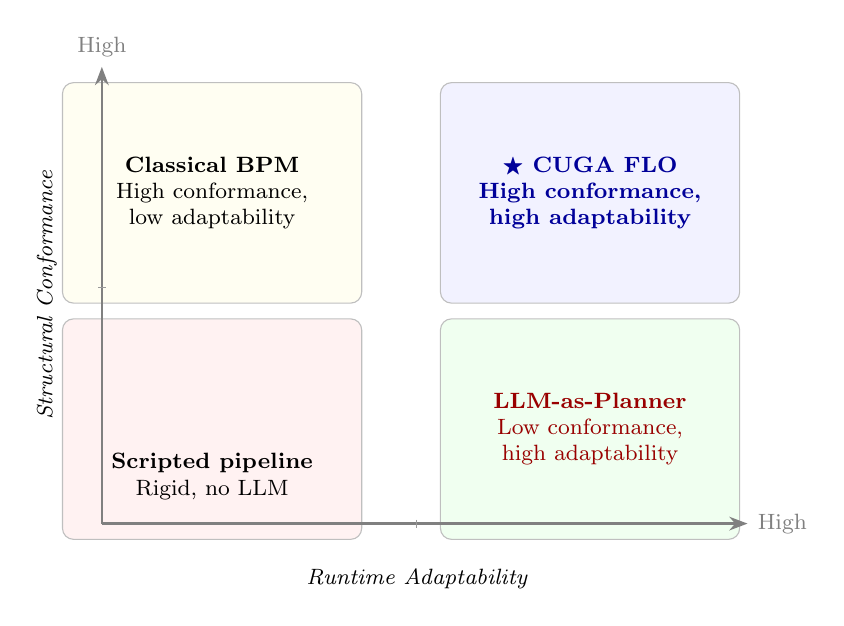
\begin{tikzpicture}[node distance=1.5cm and 2.2cm, font=\small]

% Axis labels
\node (xl) at (-0.7, 2.9) [rotate=90, anchor=center, font=\footnotesize\itshape]
      {Structural Conformance};
\node (yl) at (4, -0.7) [anchor=center, font=\footnotesize\itshape]
      {Runtime Adaptability};

% Quadrants
\node[draw=black!25, fill=red!5, minimum width=3.8cm, minimum height=2.8cm,
      rounded corners=4pt] at (1.4, 1.2) {};
\node[draw=black!25, fill=green!6, minimum width=3.8cm, minimum height=2.8cm,
      rounded corners=4pt] at (6.2, 1.2) {};
\node[draw=black!25, fill=yellow!5, minimum width=3.8cm, minimum height=2.8cm,
      rounded corners=4pt] at (1.4, 4.2) {};
\node[draw=black!25, fill=blue!5, minimum width=3.8cm, minimum height=2.8cm,
      rounded corners=4pt] at (6.2, 4.2) {};

% Axis arrows
\draw[-{Stealth}, thick, black!50] (0,0) -- (8.2,0) node[right,font=\footnotesize]{High};
\draw[-{Stealth}, thick, black!50] (0,0) -- (0,5.8) node[above,font=\footnotesize]{High};

% System labels
\node[align=center, font=\footnotesize] at (1.4, 4.2)
      {\textbf{Classical BPM}\\High conformance,\\low adaptability};
\node[align=center, font=\footnotesize\color{red!60!black}] at (6.2, 1.2)
      {\textbf{LLM-as-Planner}\\Low conformance,\\high adaptability};
\node[align=center, font=\footnotesize] at (1.4, 0.6)
      {\textbf{Scripted pipeline}\\Rigid, no LLM};
\node[align=center, font=\footnotesize\bfseries\color{blue!60!black}] at (6.2, 4.2)
      {$\bigstar$ \textbf{CUGA FLO}\\High conformance,\\high adaptability};

% Mid-axis ticks
\draw[black!40] (4, 0.05) -- (4, -0.05) node[below,font=\scriptsize]{};
\draw[black!40] (0.05, 3) -- (-0.05, 3) node[left,font=\scriptsize]{};

\end{tikzpicture}
\caption{Positioning of Agentic BPM (CUGA FLO) relative to existing approaches
along structural conformance and runtime adaptability axes.}
\label{fig:positioning}
\end{figure}

% =============================================================================
\section{The FRAME: Policy Governance in Agentic BPM}
\label{sec:frame}

\begin{definition}[FRAME]
The \emph{FRAME} of a TDF process is the aggregate set of all policy documents
governing agent reasoning within that process:
\[
  \mathcal{F} = \bigl\{\pi_T(t_i)\bigr\}_{i=1}^n \;\cup\;
                \bigl\{\pi_D(d_j)\bigr\}_{j=1}^m \;\cup\;
                \bigl\{\pi_H(h_k)\bigr\}_{k=1}^p
\]
where $\pi_T$, $\pi_D$, $\pi_H$ are task, decision, and hook policies
respectively.
\end{definition}

The FRAME serves as the \emph{policy envelope} of the process: every LLM call
in CUGA FLO is invoked with exactly one policy from the FRAME as its governing
context. No reasoning happens outside the FRAME. This creates a hierarchy of
accountability:

\begin{itemize}[noitemsep]
  \item \textbf{Task policies} $\pi_T$ specify what a task agent must accomplish,
        what process variables it must set, and what constraints it must respect.
        A task agent may not make routing decisions; its policy explicitly prohibits
        this.
  \item \textbf{Decision policies} $\pi_D$ specify the routing logic at a gateway:
        conditions, thresholds, override rules. The decision agent must return
        exactly one flow ID.
  \item \textbf{Hook policies} $\pi_H$ specify when and how the FlowAgent may
        intervene on a sequence flow: what conditions trigger intervention, what
        actions are permissible, and what process variables must be set when
        intervening.
\end{itemize}

\begin{tealframe}
\textbf{Key property.} An LLM in a CUGA FLO process can only reason about what
its assigned policy permits. A task agent cannot route. A decision agent cannot
execute domain work. A hook agent cannot modify task policies. The FRAME enforces
separation of concerns at the LLM level, not merely at the code level.
\end{tealframe}

Policies are markdown documents authored by domain experts, compliance officers,
or process designers. They are human-readable, version-controlled, and
auditable---properties absent from the gate conditions and exception handlers of
classical BPMN models.

% =============================================================================
\section{The Task--Decision--Flow Model}
\label{sec:tdf}

\subsection{Motivation and Decomposition}

The TDF model assigns LLM reasoning to exactly three node types, each with a
distinct input/output contract, quality criterion, and FRAME policy.

\begin{enumerate}[label=\textbf{(\arabic*)}, leftmargin=*, noitemsep]
  \item \textbf{TaskAgent} performs domain work: it assembles tools, reads
        process variables and prior task results, consults its task policy, and
        produces structured outputs (updated variables, reports, decisions).
        \emph{Quality criterion}: policy compliance and correctness of domain output.
  \item \textbf{DecisionAgent} performs gateway routing: it evaluates condition
        expressions against process variables using a safe analytic evaluator
        (Phase~1) and, when necessary, calls its LLM with the gateway policy
        (Phase~2) to select one outgoing flow.
        \emph{Quality criterion}: determinism and correctness of the chosen flow ID.
  \item \textbf{FlowAgent} performs meta-level process supervision: it governs the
        shared process-variable namespace, evaluates hooks at designated sequence
        flows, and reasons under hook policies to decide on structural interventions.
        It does not execute the process graph---a decoupled \texttt{WorkflowEngine}
        does, calling back into the FlowAgent at each control point through the MCP
        bridge. \emph{Quality criterion}: FRAME conformance and auditability of interventions.
\end{enumerate}

Conflating these roles is the principal failure mode of LLM-as-planner approaches:
an agent that simultaneously reasons about domain content, routing logic, and
exception handling cannot be governed by a single focused policy, and produces
brittle, non-auditable behavior.

A key design choice in the DecisionAgent is two-phase routing: for the vast
majority of arithmetic conditions encountered in real processes, Phase~1 resolves
the decision without any LLM call, making gateway routing both fast and fully
deterministic for well-specified conditions. The LLM is called in Phase~2 only
when conditions are ambiguous---for instance, when a required process variable is
absent or when the condition is a natural-language predicate.

% =============================================================================
\section{CUGA FLO: System Architecture}
\label{sec:system}

\subsection{Overview}

CUGA FLO implements the TDF model as a Python library that separates
\emph{policy-aware reasoning} from \emph{process execution}. The reasoning side---the
\texttt{FlowAgent} and its TaskAgents and DecisionAgents---is decoupled from the
execution side---a \texttt{WorkflowEngine} that drives the BPMN process graph---by
the \texttt{MCPFlowBridge}, a FastMCP server that mediates all communication between
them. The FlowAgent registers reasoning tools (\texttt{execute\_task},
\texttt{route\_gateway}, \texttt{evaluate\_hook}, \texttt{get\_static\_config}) on the
bridge; the engine calls those tools at every control point. This makes the execution
backend replaceable: the included demo engine, \texttt{LangGraphWorkflowEngine}, is
built on LangGraph, while enterprise-grade engines with their own persistence and
audit guarantees connect to the same interface without changes to the reasoning layer.
Figure~\ref{fig:architecture} shows the component architecture.

\begin{figure}[H]
\centering
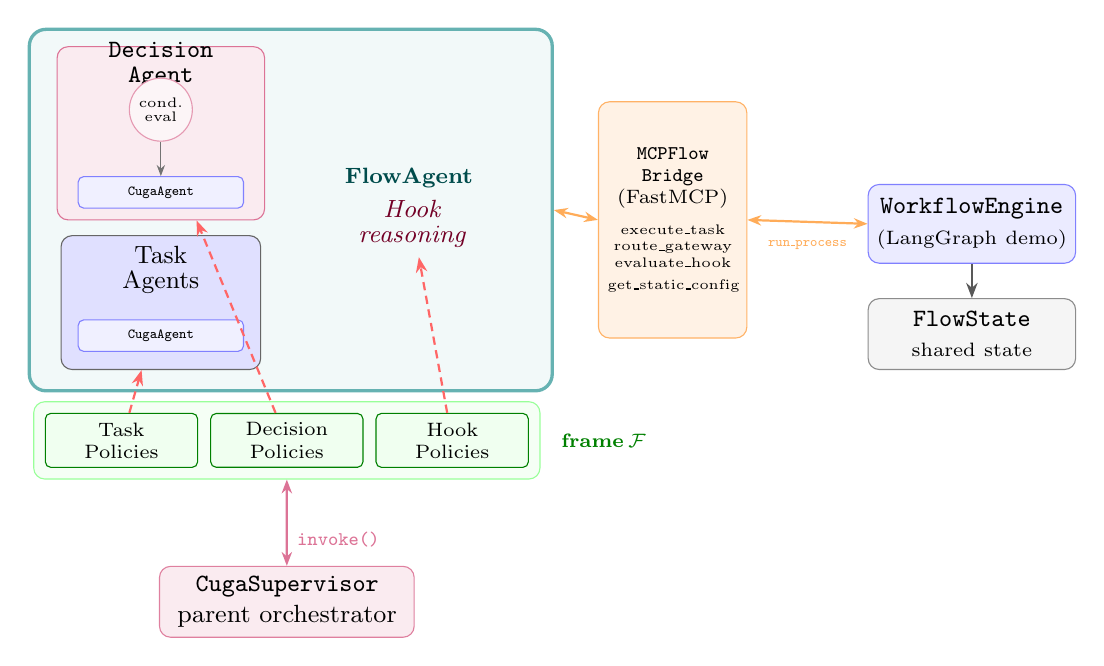
\begin{tikzpicture}[node distance=1.1cm and 1.6cm, font=\small]

% ── Reasoning side: FlowAgent box (left) ───────────────────
\coordinate (fa@bl) at (-1.0,1.65);
\coordinate (fa@tr) at (5.5,6.10);
\begin{scope}[on background layer]
  \node[frame, fit=(fa@bl)(fa@tr), inner sep=2pt] (fabox) {};
\end{scope}
\node[font=\footnotesize\bfseries\color{teal!60!black}] at (3.75,4.28)
      {FlowAgent};

% DecisionAgent outer box with condition eval circle and nested CugaAgent
\node[agent, minimum height=2.2cm] (da) at (0.6, 4.85) {};
\node[font=\small, align=center] at (0.6, 5.72) {\texttt{Decision}\\[-2pt]\texttt{Agent}};
\node[circle, draw=purple!40, fill=purple!4, minimum size=0.8cm,
      font=\tiny, align=center, inner sep=1pt] (ceval) at (0.6, 5.15)
      {cond.\\[-1pt]eval};
\node[draw=blue!50, fill=blue!6, rounded corners=2pt,
      minimum width=2.1cm, minimum height=0.4cm, font=\tiny, align=center]
      (da@ca) at (0.6, 4.10) {\texttt{CugaAgent}};
\draw[-{Stealth[length=4pt]}, thin, black!55] (ceval) -- (da@ca);

% TaskAgents outer box with nested CugaAgent
\node[task, minimum height=1.7cm] (ta) at (0.6, 2.7) {};
\node[font=\small, align=center] at (0.6, 3.12) {Task\\[-2pt]Agents};
\node[draw=blue!50, fill=blue!6, rounded corners=2pt,
      minimum width=2.1cm, minimum height=0.4cm, font=\tiny, align=center]
      at (0.6, 2.28) {\texttt{CugaAgent}};

% Hook reasoning — plain italic label inside FlowAgent, not a peer box
\node[font=\small\itshape, text centered, text width=2.0cm,
      color=purple!60!black] (hm) at (3.8, 3.7) {Hook\\[-2pt]reasoning};

% ── FRAME (below FlowAgent) ────────────────────────────────
\node[policy] (pt) at (0.1, 0.95) {Task\\Policies};
\node[policy] (pd) at (2.2, 0.95) {Decision\\Policies};
\node[policy] (ph) at (4.3, 0.95) {Hook\\Policies};
\begin{scope}[on background layer]
  \node[draw=green!40,fill=green!4,rounded corners=4pt,
        fit=(pt)(pd)(ph),inner sep=4pt] (framebox) {};
\end{scope}
\node[font=\scriptsize\bfseries\color{green!50!black}, anchor=west]
      at ([xshift=4pt]framebox.east) {\textsc{frame}\,$\mathcal{F}$};
\draw[hookflow] (pd) -- (da);
\draw[hookflow] (ph) -- (hm);
\draw[hookflow] (pt) -- (ta);

% ── MCP bridge (centre) ────────────────────────────────────
\node[draw=orange!60, fill=orange!10, rounded corners=4pt,
      minimum width=1.8cm, minimum height=3.0cm, text width=1.65cm,
      text centered, font=\scriptsize] (bridge) at (7.1,3.75)
      {\texttt{MCPFlow}\\\texttt{Bridge}\\\scriptsize(FastMCP)\\[5pt]
       \tiny execute\_task\\\tiny route\_gateway\\\tiny evaluate\_hook\\\tiny get\_static\_config};

% ── Execution side: engine and state (right) ──────────────
\node[draw=blue!50, fill=blue!8, rounded corners=4pt,
      minimum width=2.6cm, minimum height=1.0cm, text centered, text width=2.4cm]
      (engine) at (10.9,3.7) {\texttt{WorkflowEngine}\\\scriptsize(LangGraph demo)};
\node[draw=black!45, fill=gray!8, rounded corners=4pt,
      minimum width=2.6cm, minimum height=0.9cm, text centered, text width=2.4cm]
      (fs) at (10.9,2.3) {\texttt{FlowState}\\\scriptsize shared state};
\draw[flow] (engine) -- (fs);

% ── Bridge connections (bi-directional MCP) ────────────────
\draw[{Stealth[length=5pt]}-{Stealth[length=5pt]}, thick, orange!65]
      (fabox.east) -- (bridge.west);
\draw[{Stealth[length=5pt]}-{Stealth[length=5pt]}, thick, orange!65]
      (bridge.east) -- (engine.west)
      node[midway, below=3pt, font=\tiny]{\texttt{run\_process}};

% ── CugaSupervisor (bottom) ────────────────────────────────
\node[draw=purple!50, fill=purple!8, rounded corners=4pt,
      minimum width=3.2cm, minimum height=0.9cm, text centered, text width=3cm]
      (sup) at (2.2, -1.1) {\texttt{CugaSupervisor}\\parent orchestrator};

\draw[{Stealth[length=5pt]}-{Stealth[length=5pt]}, thick, purple!55]
      (framebox.south) -- (sup) node[pos=0.7, right, font=\scriptsize]{\texttt{invoke()}};

\end{tikzpicture}
\caption{CUGA FLO architecture. The reasoning side (left)---the \texttt{FlowAgent}
with its DecisionAgent, TaskAgents (each backed by a \texttt{CugaAgent}), and hook
reasoning, all governed by the FRAME $\mathcal{F}$---is decoupled from the execution
side (right) by the \texttt{MCPFlowBridge}. The bridge exposes the FlowAgent's
reasoning tools (\texttt{execute\_task}, \texttt{route\_gateway},
\texttt{evaluate\_hook}, \texttt{get\_static\_config}) and the engine's
\texttt{run\_process} tool. A replaceable \texttt{WorkflowEngine} (the included demo
is built on LangGraph) drives execution over \texttt{FlowState} and calls back into
the FlowAgent at each control point. The FlowAgent presents a unified
\texttt{invoke()} interface to a parent \texttt{CugaSupervisor}.}
\label{fig:architecture}
\end{figure}

\subsection{The FlowAgent: Process-Aware Meta-Agent}

The \texttt{FlowAgent} is the central reasoning component of CUGA FLO. It is
distinguished from a conventional LLM agent by two properties: \textbf{process-level
authority} (the FlowAgent parses the BPMN into a \texttt{BPMNProcess}, compiles the
FRAME, manages the shared process-variable namespace, and is the sole component
permitted to adapt the nominal process path---always under policy) and
\textbf{global process visibility} (during hook reasoning it receives the full
process state including, crucially, the set of remaining unexecuted task nodes,
enabling the hook LLM to reason about consequences for the \emph{remainder of the
case}).

Crucially, the FlowAgent does not execute the process graph. At initialization it
parses the BPMN, compiles each task, gateway, and hook definition into its
corresponding agent/policy structure, and registers its reasoning capabilities
(\texttt{execute\_task}, \texttt{route\_gateway}, \texttt{evaluate\_hook},
\texttt{get\_static\_config}) on the shared \texttt{MCPFlowBridge}. At runtime a
\texttt{WorkflowEngine} drives execution and invokes these tools at each control
point, passing a \texttt{ControlPointContext} that embeds the full process state,
execution history, model summary, and task instruction---so each reasoning call is
self-contained and stateless from the engine's perspective.

\paragraph{Hook-based runtime adaptation.}
Hooks are the central mechanism for runtime adaptation in CUGA FLO. In the general
model, \textbf{a hook is an annotation over a BPMN sequence flow edge}: exactly one
hook may be attached to any given edge. When execution reaches an annotated
transition, CUGA FLO intercepts it and the FlowAgent reasons---against the current
process state and the hook's policy---about how execution should proceed before the
target node is entered. Each hook carries a \texttt{location} (the flow ID it
intercepts), a \texttt{hook\_type} (one of \texttt{PRE\_EDGE}, \texttt{POST\_NODE},
\texttt{PRE\_GATEWAY}, \texttt{POST\_GATEWAY}), an optional guard \texttt{condition},
and a \texttt{policy} $\pi_H$. The FlowAgent provides to the reasoning call the
hook policy, the current process state (execution path, variables, task results),
and---uniquely---the dictionary of remaining unexecuted tasks with their BPMN IDs
and names.

The hook LLM reasons under $\pi_H$ and returns a structured action with one of
eight intervention types:

\begin{center}
\small
\begin{tabularx}{\columnwidth}{@{}llX@{}}
\toprule
\textbf{Action} & \textbf{Structural Effect} & \textbf{Semantics} \\
\midrule
\textsc{continue}
  & None (proceed normally)
  & Policy is satisfied; follow the nominal edge \\[2pt]
\textsc{skip\_node}
  & Skip the immediate next node
  & The next node records itself as skipped and control passes to its
    successor \\[2pt]
\textsc{skip\_to}
  & Jump to any named task node
  & Bypasses all intermediate nodes; target is any remaining task \\[2pt]
\textsc{swap\_nodes}
  & Exchange two nodes
  & Redirect to \texttt{node\_b} when \texttt{node\_a} was next, or to
    \texttt{node\_a} when \texttt{node\_b} was next \\[2pt]
\textsc{request\_user\_input}
  & Soft-halt; surface prompt to user
  & Pauses process; caller can resume with user reply \\[2pt]
\textsc{terminate}
  & Hard-halt the process
  & Process instance is closed; no further nodes execute \\[2pt]
\textsc{remove\_node}
  & Remove a node from the topology
  & Engine rewires the node's predecessor and successor flows to bypass it
    and resumes at the correct point \\[2pt]
\textsc{add\_node}
  & Insert a new task node
  & Engine wires flows through the new node before the current target and
    resumes at the inserted node \\
\bottomrule
\end{tabularx}
\end{center}

\medskip
The \textsc{skip\_to} action is particularly powerful: equipped with the
remaining-tasks dictionary, the hook LLM can jump to any node in the graph,
effectively reshuffling the remaining process. A hook at the midpoint of a
workflow can skip ahead to the final task or bypass multiple intermediate steps
based on a compliance condition. The first six actions are runtime navigation
decisions over the existing node set. \textsc{remove\_node} and \textsc{add\_node}
go further: they trigger a \emph{topology modification} and may only target nodes
that have not yet executed. The engine applies the structural change and resumes
execution at the correct entry point without replaying already-executed nodes.

\paragraph{Separation of concerns: instruct vs.\ execute.}
CUGA FLO issues the hook action \emph{instruction}---it does not carry it out.
Executing the action is the responsibility of the WorkflowEngine, which receives
the \texttt{HookResult} via the MCP bridge and applies the corresponding structural
intervention (routing, graph rebuild, halt) according to its own execution model.
Per-process \texttt{action\_permissions}, declared in the process configuration,
explicitly list which hook actions are permitted or prohibited for a given process,
providing an additional governance layer over what adaptations the FlowAgent may
apply. Hook reasoning is performed by the FlowAgent itself---not a separate
agent---because hooks are a process-level concern, and every deviation is
policy-governed and recorded in the audit log.

\begin{tealframe}
\textbf{LangGraph note.} In the included LangGraph engine, hooks are materialised as
intermediate graph nodes inserted at compile time between the source and target of
each annotated edge; each such node returns a \texttt{Command(goto=\ldots)} to retain
full control of the next activated node and avoid a dual-branch collision.
\textsc{remove\_node} and \textsc{add\_node} trigger a graph recompile: the hook
routes to \texttt{END}, the engine modifies the live \texttt{BPMNProcess} model,
recompiles the graph, and resumes directly at the correct entry point via a
conditional \texttt{START} edge. These choices are specific to LangGraph's compiled
graph model and are not part of the general hook contract.
\end{tealframe}

\subsection{The DecisionAgent: Policy-Governed Routing}

Each BPMN exclusive gateway that requires LLM-based routing is bound to a
\texttt{DecisionAgent}. The DecisionAgent is a specialized LLM wrapper that
implements two-phase routing.

In Phase~1, condition expressions of the form \texttt{\${var} \textgreater\
threshold} are resolved analytically by substituting process variable values and
applying Python comparison operators. No \texttt{eval()} is used, preventing code
injection. For the large majority of arithmetic conditions in real workflows,
Phase~1 is sufficient and no LLM call is made.

In Phase~2, the LLM is called with the gateway's decision policy $\pi_D$ and a
specialized \texttt{evaluate\_condition} tool. This tool is a closure over a
mutable variable dictionary that is refreshed from the process state before each
routing call, ensuring the LLM always evaluates against the current variable
values. The LLM calls the tool to obtain \texttt{TRUE}/\texttt{FALSE} for each
condition, then outputs exactly one flow ID. The response is parsed and validated
against the known outgoing flows.

\subsection{The TaskAgent: Policy-Constrained Domain Execution}

TaskAgents are \texttt{CugaAgent} instances bound to individual BPMN tasks.
Each TaskAgent receives, at invocation time, a composite input constructed by
the FlowAgent from four sources:

\begin{enumerate}[noitemsep, label=(\roman*)]
  \item The task name (from the BPMN element).
  \item The task policy $\pi_T(t_i)$ (the governing FRAME policy).
  \item The current process variables $V$ (excluding internal variables prefixed
        with \texttt{\_}).
  \item Task results from preceding tasks (\texttt{task\_results}).
\end{enumerate}

The task policy $\pi_T$ is the TaskAgent's operational specification. It specifies
what the agent must accomplish (goal), what process variables it must set (required
output), what constraints it must observe (e.g., do not approve loans—that is the
gateway's role), and what edge cases to handle. Policy compliance is the primary
quality criterion for task execution.

A TaskAgent may use any tools available in the CUGA tool registry or MCP-connected
servers. It assembles these tools autonomously under its \texttt{CugaAgent} execution
loop, returning a natural-language result. The FlowAgent extracts the output and
records it in \texttt{task\_results}, where it becomes available to subsequent nodes.

A TaskAgent additionally supports declarative \textbf{input} and \textbf{output
mappings}. An input mapping resolves named task inputs from process variables before
execution; an output mapping projects keys from the agent's structured result back
into named process variables after execution. The output mapping is what allows a
task to write process state that downstream gateways then route on---for example, a
classification task that extracts a categorical preference from a natural-language
request and writes it to a process variable consumed by an exclusive gateway.

\subsection{FlowState: Observable Shared Process State}

\texttt{FlowState} is the Pydantic state object threaded through the execution graph
and serialised across the MCP bridge. Key fields: \texttt{process\_variables} (cross-node shared store; FRAME
lingua franca), \texttt{execution\_path} (ordered activated nodes; audit trail),
\texttt{task\_results} (per-task outputs), \texttt{gateway\_decisions} (routing
audit), \texttt{hook\_evaluations} (full hook reasoning log), and halt fields
(\texttt{is\_complete}, \texttt{is\_halted}, \texttt{halt\_reason}). Process
variables are the lingua franca of the FRAME: task agents set them, decision agents
read them for routing, and hook agents read and potentially override them. All
coordination flows through this observable, serializable dictionary with no
direct inter-agent communication.

\subsection{The Integration Layer: MCP Bridge, Engine, and Registry}
\label{sec:integration}

The defining architectural choice of CUGA FLO is that the reasoning layer (the
FlowAgent and its sub-agents) and the execution layer (the workflow engine) are
fully decoupled and communicate only through a Model Context Protocol bridge. This
makes the execution backend replaceable without any change to the reasoning layer.
The runtime interaction sequence is shown in Figure~\ref{fig:sequence}.

\paragraph{MCPFlowBridge.}
The \texttt{MCPFlowBridge} is a FastMCP server that acts as the integration contract
between the FlowAgent harness and any \texttt{WorkflowEngine}. The FlowAgent side
registers four reasoning tools---\texttt{execute\_task} (a BPMN task node is
reached), \texttt{route\_gateway} (a gateway needs a routing decision),
\texttt{evaluate\_hook} (a hook intercept point fires), and
\texttt{get\_static\_config} (the engine fetches process metadata at startup). The
engine side registers \texttt{run\_process} (start a new process instance). Every
call carries a \texttt{ControlPointContext}, so each reasoning call is self-contained
and the engine is stateless from the FlowAgent's perspective. A remote transport
(HTTP/SSE) can be substituted for the in-process transport without changing either
side, enabling cross-process or cross-host deployment.

\paragraph{WorkflowEngine.}
The \texttt{WorkflowEngine} is the abstract execution backend. It holds the process
model and instance state, drives execution node by node, and communicates with the
FlowAgent exclusively through the bridge---calling the corresponding reasoning tool
at each control point. The included demo engine, \texttt{LangGraphWorkflowEngine},
compiles the BPMN topology into a LangGraph \texttt{StateGraph}; enterprise-grade
engines with their own persistence, audit trails, and compliance guarantees connect
to the same interface in production. This is the sense in which the structural
conformance guarantee of CUGA FLO is engine-enforced: the engine executes the actual
BPMN topology, and the FlowAgent governs only the policy-bounded reasoning at
designated control points.

\paragraph{ProcessRegistry.}
The \texttt{ProcessRegistry} is a catalog of BPMN process definitions, mapping short
process keys to a parsed \texttt{BPMNProcess} paired with its \texttt{FlowConfig}, and
caching parsed results for reuse across invocations. It auto-discovers process
definitions from a directory, allowing a single deployment to serve many distinct
processes through one bridge.

Figure~\ref{fig:sequence} shows the runtime interaction sequence.

\begin{figure}[H]
\centering
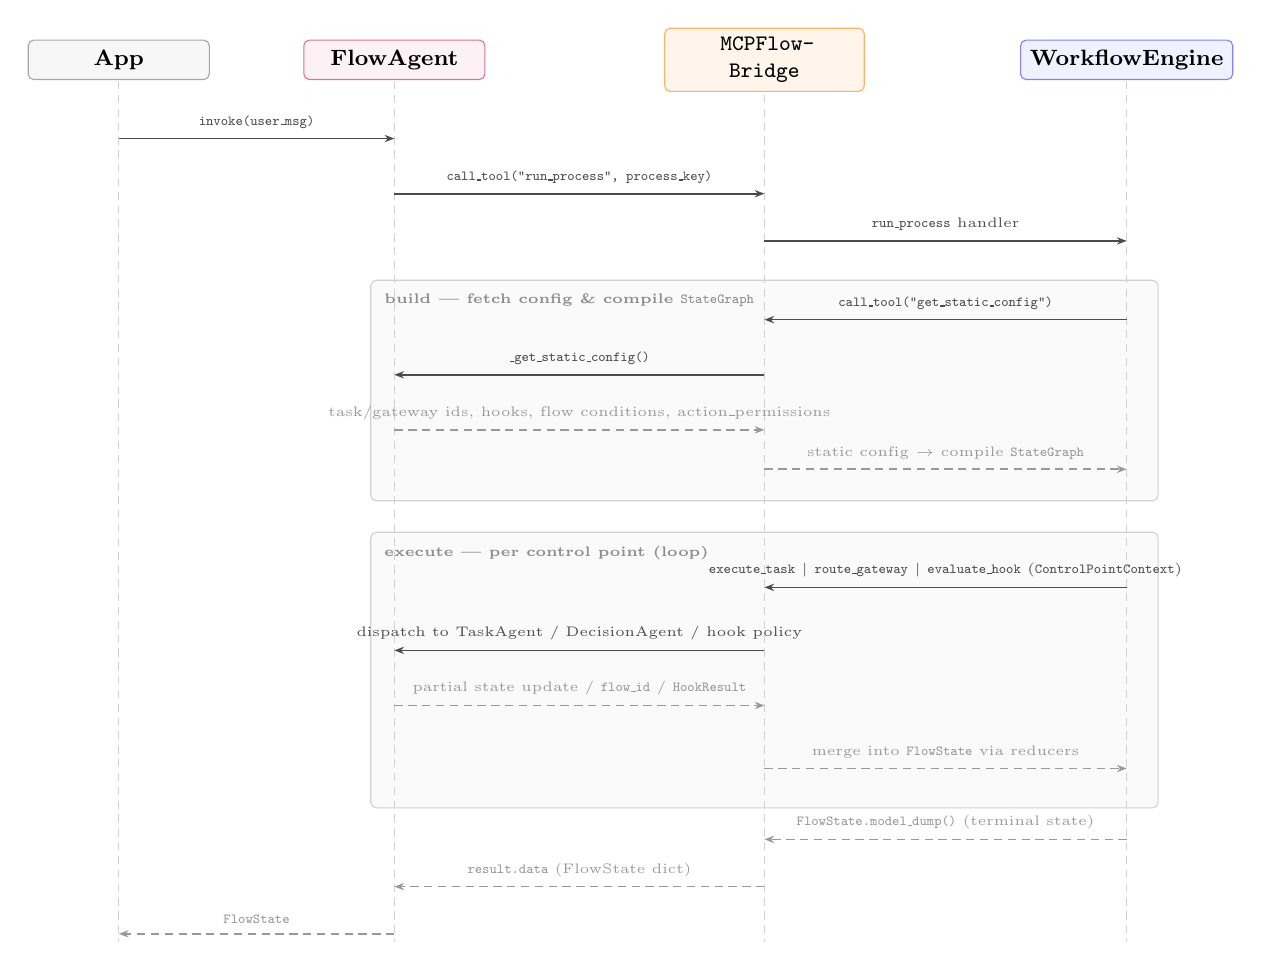
\begin{tikzpicture}[
  seqact/.style={rectangle, rounded corners=2pt, draw=black!50,
                 minimum width=2.3cm, minimum height=0.5cm,
                 text centered, font=\footnotesize\bfseries, fill=white},
  msg/.style={-{Stealth[length=3.5pt]}, semithick, black!70},
  ret/.style={-{Stealth[length=3.5pt]}, semithick, black!40, densely dashed},
]

%% Lifeline x-positions
\def\xA{0}     % App
\def\xF{3.5}   % FlowAgent
\def\xB{8.2}   % MCPFlowBridge
\def\xE{12.8}  % WorkflowEngine

%% Phase background boxes (drawn first so they sit behind everything)
\begin{scope}[on background layer]
  \draw[rounded corners=2pt, draw=black!18, fill=gray!4]
       (\xF-0.3,-2.8) rectangle (\xE+0.4,-5.6);
  \draw[rounded corners=2pt, draw=black!18, fill=gray!4]
       (\xF-0.3,-6.0) rectangle (\xE+0.4,-9.5);
\end{scope}

%% Phase labels
\node[font=\tiny\bfseries\color{black!45}, anchor=north west]
     at (\xF-0.25,-2.85) {build — fetch config \& compile \texttt{StateGraph}};
\node[font=\tiny\bfseries\color{black!45}, anchor=north west]
     at (\xF-0.25,-6.05) {execute — per control point (loop)};

%% Lifelines
\draw[black!18, densely dashed, thin] (\xA,-0.27) -- (\xA,-11.2);
\draw[black!18, densely dashed, thin] (\xF,-0.27) -- (\xF,-11.2);
\draw[black!18, densely dashed, thin] (\xB,-0.27) -- (\xB,-11.2);
\draw[black!18, densely dashed, thin] (\xE,-0.27) -- (\xE,-11.2);

%% Participant headers
\node[seqact, draw=black!35,   fill=gray!6]    at (\xA,0) {App};
\node[seqact, draw=purple!55,  fill=purple!5]  at (\xF,0) {FlowAgent};
\node[seqact, draw=orange!60,  fill=orange!8,  text width=2.3cm]
     at (\xB,0) {\texttt{MCPFlow-}\\\texttt{Bridge}};
\node[seqact, draw=blue!50,    fill=blue!6]    at (\xE,0) {WorkflowEngine};

%% ── (1) App invokes FlowAgent ───────────────────────────────────────────
\draw[msg] (\xA,-1.0) -- (\xF,-1.0)
     node[midway,above,font=\tiny]{\texttt{invoke(user\_msg)}};

%% ── (2) FlowAgent calls run_process via bridge ─────────────────────────
\draw[msg] (\xF,-1.7) -- (\xB,-1.7)
     node[midway,above,font=\tiny]{\texttt{call\_tool("run\_process", process\_key)}};
\draw[msg] (\xB,-2.3) -- (\xE,-2.3)
     node[midway,above,font=\tiny]{\texttt{run\_process} handler};

%% ── BUILD phase ─────────────────────────────────────────────────────────
%% Engine fetches static config from FlowAgent via bridge
\draw[msg] (\xE,-3.3) -- (\xB,-3.3)
     node[midway,above,font=\tiny]{\texttt{call\_tool("get\_static\_config")}};
\draw[msg] (\xB,-4.0) -- (\xF,-4.0)
     node[midway,above,font=\tiny]{\texttt{\_get\_static\_config()}};
\draw[ret] (\xF,-4.7) -- (\xB,-4.7)
     node[midway,above,font=\tiny]{task/gateway ids, hooks, flow conditions, action\_permissions};
\draw[ret] (\xB,-5.2) -- (\xE,-5.2)
     node[midway,above,font=\tiny]{static config $\rightarrow$ compile \texttt{StateGraph}};

%% ── EXECUTE phase ───────────────────────────────────────────────────────
%% Engine calls FlowAgent reasoning tools at each BPMN control point
\draw[msg] (\xE,-6.7) -- (\xB,-6.7)
     node[midway,above,font=\tiny]{\texttt{execute\_task} $|$ \texttt{route\_gateway} $|$ \texttt{evaluate\_hook}
     (\texttt{ControlPointContext})};
\draw[msg] (\xB,-7.5) -- (\xF,-7.5)
     node[midway,above,font=\tiny]{dispatch to TaskAgent / DecisionAgent / hook policy};
\draw[ret] (\xF,-8.2) -- (\xB,-8.2)
     node[midway,above,font=\tiny]{partial state update / \texttt{flow\_id} / \texttt{HookResult}};
\draw[ret] (\xB,-9.0) -- (\xE,-9.0)
     node[midway,above,font=\tiny]{merge into \texttt{FlowState} via reducers};

%% ── COMPLETE ────────────────────────────────────────────────────────────
\draw[ret] (\xE,-9.9) -- (\xB,-9.9)
     node[midway,above,font=\tiny]{\texttt{FlowState.model\_dump()} (terminal state)};
\draw[ret] (\xB,-10.5) -- (\xF,-10.5)
     node[midway,above,font=\tiny]{\texttt{result.data} (FlowState dict)};
\draw[ret] (\xF,-11.1) -- (\xA,-11.1)
     node[midway,above,font=\tiny]{\texttt{FlowState}};

\end{tikzpicture}
\caption{CUGA FLO runtime interaction sequence. Solid arrows are calls; dashed
arrows are returns. \texttt{MCPFlowBridge} is the sole channel between the reasoning
layer (\texttt{FlowAgent}) and the execution layer (\texttt{WorkflowEngine}).
The \emph{build} phase (once per invocation) fetches static config so the engine can
compile its LangGraph \texttt{StateGraph}. The \emph{execute} phase issues one
round-trip per BPMN control point---task nodes, gateways, and hook intercept
edges---passing a \texttt{ControlPointContext} and receiving structured results that
the engine merges into \texttt{FlowState}. No direct reference between
\texttt{FlowAgent} and \texttt{WorkflowEngine} exists; either side can be replaced by
swapping the transport or the engine implementation.}
\label{fig:sequence}
\end{figure}

% =============================================================================
\section{Comparison with Related Paradigms}
\label{sec:comparison}

\subsection{Property Analysis}

We compare CUGA FLO against three reference systems along three properties.

\begin{table}[H]
\centering
\small
\begin{tabularx}{\textwidth}{@{}Xcccc@{}}
\toprule
\textbf{Property} &
\textbf{Classical BPM} &
\textbf{LLM-as-Planner} &
\textbf{ReAct/AutoGen} &
\textbf{CUGA FLO (TDF)} \\
\midrule
BPMN process graph & \checkmark & Input only & \texttimes & \checkmark (executed) \\
Structural conformance & \checkmark & \texttimes & \texttimes & \checkmark \\
Runtime adaptability & \texttimes & \checkmark & \checkmark & \checkmark \\
Human-readable policies & \texttimes & \texttimes & \texttimes & \checkmark \\
Policy accountability & \texttimes & \texttimes & \texttimes & \checkmark \\
Audit trail (per element) & \checkmark & \texttimes & \texttimes & \checkmark \\
Exception: design-time & \checkmark & \texttimes & \texttimes & Optional \\
Exception: open-world & \texttimes & \checkmark & \checkmark & \checkmark \\
Repeatable traces & \checkmark & \texttimes & \texttimes & \checkmark \\
Non-programmer authoring & \texttimes & \texttimes & \texttimes & \checkmark \\
\bottomrule
\end{tabularx}
\caption{Property comparison across process execution paradigms.}
\label{tab:comparison}
\end{table}

\subsection{The Key Distinctions}

\paragraph{vs.\ Classical BPM exception handling.}
Classical BPM exception handling is \emph{additive} and \emph{design-time}: every
deviation path must be pre-modeled as a boundary event, error sub-process, or
compensation handler. CUGA FLO hooks are \emph{open-world}: the set of situations
a hook policy can handle is the set of situations the policy document can reason
about. In the loan example, the regulatory rule is a markdown policy reasoned about
per case---not a diagram element. Adding a new exception in classical BPM requires
a diagram change (release-gated); in CUGA FLO it is a policy document update.

\paragraph{vs.\ LLM-as-Planner.}
LLM-as-planner treats the BPMN as \emph{input}: the LLM reads it and constructs
an ad~hoc plan without enforcement. CUGA FLO is fundamentally different: the
workflow engine executes the BPMN topology directly, making non-conforming
execution physically impossible; adaptations
happen at runtime with actual process state (not predicted context); and every
activated node, gateway decision, and hook evaluation is recorded in \texttt{FlowState}
tied to BPMN element IDs. Two planning-LLM invocations with identical inputs may
produce structurally different traces; CUGA FLO traces are structurally determined
by the BPMN graph.

\begin{remark}[Adaptive Conformance]
Hook-driven redirects, skips, and jumps are not violations of the process model.
They are runtime selections among nodes that exist in the process graph; even the
topology-modifying actions produce, after the engine applies them, a graph whose
nodes are well-formed BPMN elements. Every such deviation is policy-bounded and
recorded in the audit trail.
\end{remark}

% =============================================================================
\section{Case Study: Loan Approval Workflow}
\label{sec:casestudy}

\subsection{Process Overview}

We demonstrate CUGA FLO through a loan approval workflow that instantiates all
three TDF agent types. The workflow evaluates personal loan applications in four
stages: credit assessment, approval routing, outcome handling, and merge.

\subsubsection{BPMN Structure}

\begin{figure}[H]
\centering
\resizebox{\linewidth}{!}{\begin{tikzpicture}[node distance=0.7cm and 1.4cm]

\node[event] (start) {S};

\node[task, right=1.2cm of start, yshift=0pt] (credit)
      {Check\\Credit\\{\scriptsize\color{purple!70}TaskAgent}};

\node[gateway, right=1.5cm of credit] (gw1) {XOR};
\node[font=\scriptsize, above=0.3cm of gw1, xshift=0.2cm, color=black!55]
      {\texttt{\$\{credit\_score\}~>~0.6}};
\node[font=\scriptsize, right=0.1cm of gw1, yshift=-0.75cm, color=purple!60]
      {DecisionAgent};

% Hook node on "yes" branch
\node[hook, right=0.9cm of gw1, yshift=1.2cm] (hook)
      {Hook:\\audit\_credit};

\node[task, right=1.1cm of hook] (loan)
      {Give Loan\\(\$1{,}000)\\{\scriptsize\color{purple!70}TaskAgent}};

\node[task, right=0.9cm of gw1, yshift=-1.2cm] (reject)
      {Send\\Rejection\\{\scriptsize\color{purple!70}TaskAgent}};

\node[gateway, right=1.5cm of loan, yshift=-1.2cm] (gw2) {XOR};

\node[event, right=1.2cm of gw2] (end) {E};

% Nominal flows
\draw[flow] (start) -- (credit);
\draw[flow] (credit) -- (gw1);
\draw[hookflow] (gw1.north) -- ++(0,0.45) -- node[above,font=\scriptsize]{yes} (hook.west);
\draw[hookflow] (hook) -- (loan);
\draw[flow] (gw1.south) -- ++(0,-0.35) -- node[above,font=\scriptsize]{no} (reject.west);
\draw[flow] (loan.east) -| (gw2.north);
\draw[flow] (reject.east) -| (gw2.south);
\draw[flow] (gw2) -- (end);

% Hook override annotation
\draw[-{Stealth[length=4pt]}, red!55, thick, dashed, bend right=20]
      (hook.south east) to node[right, align=left, font=\scriptsize\color{red!60}]
      {override\\(ID 4321)} (reject.north east);

\end{tikzpicture}}
\caption{Loan approval BPMN diagram with TDF annotations. The red dashed hook
node intercepts the ``yes'' sequence flow (\texttt{Flow\_0ybszcv}); the curved
red arrow shows the \textsc{skip\_to} redirect for applicant ID~4321.}
\label{fig:bpmn}
\end{figure}

\subsection{FRAME Instantiation}

The FRAME $\mathcal{F}$ for this process comprises four policy documents:

\subsubsection{Task Policy: Credit Check}

\begin{policybox}
\textbf{Credit Check Policy (abbreviated).}
Analyse the applicant's financial profile and produce a normalised
\texttt{credit\_score} $\in [0,1]$. Score using: payment history (35\%),
debt-to-income (30\%), history length (15\%), credit mix (10\%), recent
enquiries (10\%). Set \texttt{credit\_score} before completing. \emph{Do not
approve or reject---that belongs to the gateway.}
\end{policybox}

The explicit prohibition ``do not approve or reject'' is the policy-level
enforcement of TDF separation: the task agent is constrained from performing
gateway routing, even though it has the credit score value.

\subsubsection{Decision Policy: Credit Gateway}

\begin{policybox}
\textbf{Decision Policy: Gateway\_09ad5fc.}
Route using \texttt{\${credit\_score} > 0.6}: scores above 0.60 to the
approval path (\texttt{Flow\_0ybszcv}); at or below to rejection
(\texttt{Flow\_1jgea85}). Override: if \texttt{loan\_amount > 50{,}000} apply
strict threshold 0.75. Output exactly one flow ID.
\end{policybox}

For the typical case (\texttt{credit\_score} is a float), Phase~1 resolves this
deterministically. The LLM is called
only when \texttt{credit\_score} is absent or the higher threshold override
applies.

\subsubsection{Hook Policy: Regulatory Override}

\begin{policybox}
\textbf{Hook Policy: audit\_credit\_decision.}
\textbf{Rule}: Applicant ID \texttt{4321} is subject to regulatory restriction;
redirect to rejection. Set \texttt{rejection\_reason =}\\
\texttt{"regulatory\_policy\_restriction"}\\
and \texttt{policy\_override\_active = true}.
\textbf{Default}: All other IDs---return \textsc{continue} with no state
updates.
\end{policybox}

\subsubsection{Task Policies: Outcome Handling}

\begin{sloppypar}
The loan processor policy requires: verify \texttt{approved == true}
before disbursing; set \texttt{loan\_granted = true}; do not send rejections.
The rejection handler policy routes between two paths based on
\texttt{rejection\_reason}: standard credit-score rejection or regulatory
override path (never reference the credit score; cite regulatory compliance).
\end{sloppypar}

\subsection{Execution Traces}

\paragraph{Nominal case (ID~23, score~0.6625).}
\begin{enumerate}[noitemsep, label=\arabic*.]
  \item TaskAgent: credit check → \texttt{credit\_score = 0.6625}
  \item DecisionAgent: Phase-1 eval of \texttt{0.6625 > 0.6} → \texttt{TRUE}
        → record \texttt{Flow\_0ybszcv}
  \item Hook (ID~23): LLM evaluates policy → \textsc{continue} → proceed to
        loan processing
  \item TaskAgent: loan processor → \texttt{loan\_granted = true}
\end{enumerate}

\paragraph{Regulatory block (ID~4321, score~0.82).}
\begin{enumerate}[noitemsep, label=\arabic*.]
  \item TaskAgent: credit check → \texttt{credit\_score = 0.82}
  \item DecisionAgent: Phase-1 eval → \texttt{TRUE} → record \texttt{Flow\_0ybszcv}
  \item Hook (ID~4321): LLM evaluates policy → \textsc{skip\_to}
        \texttt{Activity\_131ar38};\\
        patches \texttt{rejection\_reason =}
        \texttt{"regulatory\_policy\_restriction"}
  \item TaskAgent: rejection handler → regulatory path (no credit score reference)
\end{enumerate}

This trace illustrates the core Agentic BPM property: the DecisionAgent routes
correctly by credit score (0.82 \textgreater\ 0.6), while the hook overrides
the resulting edge based on a wholly different criterion (applicant ID)---without
modifying the gateway policy. The two concerns are independently governed by
separate FRAME policies, each auditable in isolation.

\subsection{FlowAgent Instantiation}

\begin{lstlisting}[style=python, caption={Complete FlowAgent instantiation for the loan approval workflow.}]
loan_flow_agent = FlowAgent(
    bpmn_file=str(CONFIG / "BPMNdiagram.bpmn"),
    task_agents={
        "Activity_0oydey5": credit_checker_agent,    # Check Credit
        "Activity_1h9ix55": loan_processor_agent,    # Give Loan
        "Activity_131ar38": rejection_handler_agent, # Send Rejection
    },
    task_policies={
        "Activity_0oydey5": (POLICIES/"task-credit_check.md").read_text(),
        "Activity_1h9ix55": (POLICIES/"task-loan_processor.md").read_text(),
        "Activity_131ar38": (POLICIES/"task-rejection_handler.md").read_text(),
    },
    gateway_agents={
        # Gateway_15y9k7z (merge) uses tool-mode: single outgoing flow
        "Gateway_09ad5fc": DecisionAgent(
            gateway_id="Gateway_09ad5fc",
            policy=(POLICIES/"decision-credit_decision.md").read_text(),
            condition="${credit_score} > 0.6",
            flow_decisions={
                "Flow_0ybszcv": "Approve -- credit score sufficient",
                "Flow_1jgea85": "Reject -- credit score insufficient",
            },
        ),
    },
    process_variables={
        "applicant_name": "", "applicant_id": "",
        "loan_amount": 1000, "credit_score": 0.0, "approved": False,
    },
    hooks=[
        Hook(
            id="audit_credit_decision",
            hook_type=HookType.PRE_EDGE,
            location="Flow_0ybszcv",          # "yes" arc only
            handler=lambda state: HookResult(action=HookAction.CONTINUE),
            policy=(POLICIES/"hook-audit_credit_decision.md").read_text(),
        ),
    ],
)
\end{lstlisting}

Several design points merit comment. The merge gateway
(\texttt{Gateway\_15y9k7z}) has a single outgoing flow and is handled in
``tool mode''---no DecisionAgent is instantiated, and no LLM call is made at
that node. The hook is attached exclusively to \texttt{Flow\_0ybszcv} (the
``yes'' arc), so it fires only when the credit decision would result in approval;
the rejection path bypasses the hook entirely. The \texttt{handler} lambda
provides a fallback for non-policy invocations; the \texttt{policy} field
activates LLM reasoning.

% =============================================================================
\section{Discussion}
\label{sec:discussion}

\subsection{Novelty of the Agentic BPM Paradigm}

CUGA FLO is, to our knowledge, the first system to embed LLM agents as
policy-bounded \emph{governing authorities} over a BPMN execution graph rather than
as consumers of a BPMN description. Classical BPM exception handling is
\emph{additive}: exceptions add elements to the diagram. Agentic BPM exception
handling is \emph{interceptive}: hooks annotate existing sequence flows and reason
about them at runtime using natural-language policies that can handle nuance without
enumerating cases at design time. Navigation actions select among valid BPMN nodes
in the process graph, while topology actions (node insertion and removal) modify the
graph under policy and are then executed by the engine---so the mechanism is
genuinely open-world while remaining structurally sound and auditable.

The FRAME $\mathcal{F}$ provides an accountability substrate absent from
LLM-as-planner approaches: every LLM call can be audited against its governing
policy document, and non-compliance is diagnosable without inspecting code.

\subsection{Limitations and Future Work}

\paragraph{BPMN coverage and graph modification.}
The current implementation handles tasks, exclusive and parallel gateways, and
sequence flows. Intermediate events, event sub-processes, and timer events are not
yet supported. Runtime topology modification---inserting or removing a task node
relative to the original BPMN---is supported through the \textsc{add\_node} and
\textsc{remove\_node} hook actions: the engine modifies the live process model,
recompiles, and resumes at the correct entry point without replaying already-executed
nodes (such modifications may only target nodes that have not yet executed). Lifting
this not-yet-executed restriction, and supporting modification of in-flight parallel
branches, remains future work.

\paragraph{Hook cost and FRAME authoring.}
Policy-driven hooks invoke an LLM on every traversal of their attached flow,
introducing per-instance latency proportional to hook count. Caching decisions for
recurring state patterns or using lightweight pre-filter classifiers are promising
mitigations. Authoring a complete FRAME also requires care: conflicting policies
across task, decision, and hook documents may produce incoherent behavior.
Automated FRAME consistency checking---analogous to static analysis of classical
BPM models---is an important open problem.

% =============================================================================
\section{Related Work}
\label{sec:related}

\paragraph{LLM agents, planning, and workflow automation.}
ReAct~\cite{yao2022react} interleaves reasoning and tool use; we adopt tool-call
patterns for DecisionAgent routing. AutoGen~\cite{wu2023autogen} and
CrewAI~\cite{crewai2024} organize role-specialized agents; TDF provides a formal
semantic layer for such roles. LLM-based planning~\cite{kambhampati2024llm}
identifies plan correctness as an open problem that TDF's structural conformance
addresses. RPA executes scripted bots within BPMN structures; CUGA FLO replaces
them with LLM agents while preserving structural guarantees. Conversational
workflow systems~\cite{qian2024chatdev} coordinate agents through dialogue; TDF
uses a compiled graph for stronger ordering guarantees.

\paragraph{Policy, governance, and process-aware AI.}
Constitutional AI~\cite{bai2022constitutional} and rule-based
constraints~\cite{perez2021selfdiagnosis} study policy-governed AI; CUGA FLO
operationalizes governance at the process level via the FRAME. Intelligent process
automation~\cite{geyer2021intelligent} uses ML for decision support; CUGA FLO
makes the agent the process executor. Adaptive case
management~\cite{swenson2010mastering} addresses flexible processes; Agentic BPM
replaces rule-based adaptation with LLM reasoning bounded by the FRAME.

\paragraph{From AI-augmented to Agentic BPM.}
The trajectory of research leading to CUGA FLO follows a clear paradigm
progression. Dumas et al.~\cite{dumas2023aiaugmented} introduced the AI-augmented
BPM (ABPMS) vision, in which AI capabilities are embedded into BPM systems to
make processes more adaptive, proactive, and context-sensitive. This laid the
foundation for the \emph{Agentic BPM} paradigm, formally articulated as a
research manifesto in~\cite{calvanese2026agenticbpm}: agents act as primary
functional entities that perceive, reason, and act within explicit process frames,
with framed autonomy, explainability, and conversational actionability as core
capabilities. An architectural vision for Agentic BPMSs is further developed
in~\cite{dumas2026abpms}.

\paragraph{Agent-centric as successor to object-centric.}
This progression also reflects a broader shift in process management paradigms.
Object-centric BPM~\cite{vanderaalst2026objectcentric} challenged the traditional
case-centric assumption by placing \emph{objects}---co-evolving data entities---at
the center of process analysis and execution. Agentic BPM takes the next step:
it places \emph{agents} as the core functional entities driving the process.
Just as object-centricity expanded the unit of analysis from a single case token
to a network of interacting objects, agent-centricity expands it further to
autonomous reasoning entities that perceive state, consult policies, and act
within a structural process frame. CUGA FLO operationalizes this vision through
the TDF model and the FRAME.

% =============================================================================
\section{Conclusion}
\label{sec:conclusion}

We have presented CUGA FLO, the first realization of Agentic BPM, and the
Task--Decision--Flow (TDF) model that governs it. The central insight is that
structured process execution and open-world adaptability are not in fundamental
tension: they require a process-aware, policy-aware agent that governs the process
---the FlowAgent---and a principled mechanism for runtime structural
intervention---hooks governed by the FRAME. A Model Context Protocol bridge
(\texttt{MCPFlowBridge}) decouples this reasoning authority from a replaceable
workflow execution engine, so that structural conformance is engine-enforced while
adaptation remains policy-bounded.

The TDF model decomposes LLM reasoning across three agent types with distinct
contracts: TaskAgents assemble tools to perform domain work under task policies;
DecisionAgents evaluate gateway conditions under decision policies with a
deterministic first pass; and the FlowAgent reasons at the meta-level under hook
policies to decide on structural interventions ranging from simple continues to
runtime modification of the process topology.

The FRAME---the aggregate policy set---provides an accountability substrate absent
from LLM-as-planner approaches: every LLM call is auditable against its governing
policy document, and non-compliance is diagnosable without inspecting code.

Compared to classical BPM exception handling, hooks provide an open-world
adaptation mechanism that does not require anticipating exceptions at design time.
Compared to LLM-as-planner approaches, structural fidelity is guaranteed by
construction: the workflow engine executes the BPMN topology directly, and the
FlowAgent may deviate only through policy-bounded hook actions whose permitted set
is explicitly declared per process.

The loan approval case study instantiates all three agent types and demonstrates
regulatory override through hook-driven \textsc{skip\_to}, with the FlowAgent
reasoning about the full remaining task set to identify the correct jump target.
The mechanism is transparent, auditable, and governed at every step by the FRAME.

We believe Agentic BPM represents a significant step towards enterprise-grade
AI process execution, combining the structural rigour of process management with
the open-ended reasoning of modern LLMs. The CUGA FLO codebase, including all
policies and the loan approval example, is provided as an open reference
implementation.

% =============================================================================
\bibliographystyle{plain}
\begin{thebibliography}{99}

\bibitem{vdaalst2016processm}
W.\ M.\ P.\ van der Aalst,
\emph{Process Mining: Data Science in Action}, 2nd ed.
Springer, Berlin, 2016.

\bibitem{bpmn2011}
Object Management Group,
\emph{Business Process Model and Notation (BPMN) Version 2.0},
OMG Document formal/2011-01-03, 2011.

\bibitem{yao2022react}
S.\ Yao, J.\ Zhao, D.\ Yu, N.\ Du, I.\ Shafran, K.\ Narasimhan, and Y.\ Cao,
``ReAct: Synergizing Reasoning and Acting in Language Models,''
in \emph{Proc.\ ICLR}, 2023.

\bibitem{wang2024survey}
L.\ Wang et al.,
``A Survey on Large Language Model based Autonomous Agents,''
\emph{Frontiers of Computer Science}, vol.\ 18, no.\ 6, 2024.

\bibitem{wu2023autogen}
Q.\ Wu, G.\ Bansal, J.\ Zhang, Y.\ Wu, S.\ Zhang, E.\ Zhu, B.\ Li,
L.\ Jiang, X.\ Zhang, and C.\ V.\ Wang,
``AutoGen: Enabling Next-Gen LLM Applications via Multi-Agent Conversation,''
\emph{arXiv preprint arXiv:2308.08155}, 2023.

\bibitem{crewai2024}
J.\ Moura,
``CrewAI: Framework for Orchestrating Role-Playing Autonomous AI Agents,''
\url{https://github.com/joaomdmoura/crewAI}, 2024.

\bibitem{langgraph2024}
LangChain AI,
``LangGraph: Build Stateful, Multi-Actor Applications with LLMs,''
\url{https://github.com/langchain-ai/langgraph}, 2024.

\bibitem{kambhampati2024llm}
S.\ Kambhampati, K.\ Valmeekam, L.\ Guan, K.\ Stechly, M.\ Verma,
S.\ Bhambri, L.\ Saldyt, and A.\ Murthy,
``LLMs Can't Plan, But Can Help Planning in LLM-Modulo Frameworks,''
\emph{arXiv preprint arXiv:2402.01817}, 2024.

\bibitem{deng2023mind2web}
X.\ Deng, Y.\ Gu, B.\ Zheng, S.\ Chen, S.\ Stevens, B.\ Wang, H.\ Sun,
and Y.\ Su,
``Mind2Web: Towards a Generalist Agent for the Web,''
in \emph{Proc.\ NeurIPS}, 2023.

\bibitem{bai2022constitutional}
Y.\ Bai et al.,
``Constitutional AI: Harmlessness from AI Feedback,''
\emph{arXiv preprint arXiv:2212.08073}, 2022.

\bibitem{qian2024chatdev}
C.\ Qian et al.,
``Communicative Agents for Software Development,''
in \emph{Proc.\ ACL}, 2024.

\bibitem{swenson2010mastering}
K.\ D.\ Swenson,
\emph{Mastering the Unpredictable: How Adaptive Case Management Will
Revolutionize the Way That Knowledge Workers Get Things Done},
Meghan-Kiffer Press, 2010.

\bibitem{geyer2021intelligent}
R.\ Geyer-Klingeberg, M.\ Nakladal, F.\ Vollmann, and F.\ Vogt,
``Process Mining and Robotic Process Automation: A Perfect Match,''
in \emph{Proc.\ CEUR Workshop}, 2021.

\bibitem{perez2021selfdiagnosis}
E.\ Perez, S.\ Huang, F.\ Song, T.\ Cai, R.\ Ring, J.\ Aslanides,
A.\ Askell, N.\ Baughman, and G.\ Irving,
``Red Teaming Language Models with Language Models,''
\emph{arXiv preprint arXiv:2202.03286}, 2022.

\bibitem{dumas2023aiaugmented}
M.\ Dumas, F.\ Fournier, L.\ Limonad, A.\ Marrella, M.\ Montali,
J.\ R.\ Rehse, R.\ Accorsi, D.\ Calvanese, G.\ De Giacomo,
D.\ Fahland, A.\ Gal, M.\ La Rosa, H.\ V\"olzer, and I.\ Weber,
``AI-augmented Business Process Management Systems: A Research Manifesto,''
\emph{ACM Transactions on Management Information Systems},
vol.\ 14, no.\ 1, art.\ 11, 2023.

\bibitem{calvanese2026agenticbpm}
D.\ Calvanese, A.\ Casciani, G.\ De Giacomo, M.\ Dumas, F.\ Fournier,
T.\ Kampik, E.\ La Malfa, L.\ Limonad, A.\ Marrella, A.\ Metzger,
M.\ Montali et al.,
``Agentic Business Process Management: A Research Manifesto,''
\emph{Information Systems}, 2026.
arXiv preprint arXiv:2603.18916.

\bibitem{dumas2026abpms}
M.\ Dumas, F.\ Milani, and D.\ Chapela-Campa,
``Agentic Business Process Management Systems,''
in \emph{Business Process Management Workshops: BPM 2025
International Workshops, Seville, Spain, Revised Selected Papers},
Springer, 2026, ch.\ 1.
arXiv preprint arXiv:2601.18833.

\bibitem{vanderaalst2026objectcentric}
W.\ M.\ P.\ van der Aalst et al.,
``Object-centric Process Management: A Research Manifesto,''
\emph{Information Systems}, 2026.

\end{thebibliography}

\end{document}
